\qrchapter{https://forgottenpillar.com/rsc/en-fp-chapter1}{The historical context}


\qrchapter{https://forgottenpillar.com/rsc/en-fp-chapter1}{السياق التاريخي}


Ellen White recalled encountering the same sentiments in \textit{The Living Temple} that she had warned against early in her ministry:


تذكرت إلين وايت أنها واجهت نفس الآراء في \textit{ذا ليفينغ تمبل} التي حذرت منها في بداية خدمتها:


\egw{As we read \normaltext{[The Living Temple]}, I recognized the very sentiments against which I had been bidden to speak in warning \textbf{during the early days of my public labors}. \textbf{When I first left \underline{the State of Maine, it was to go through Vermont and Massachusetts}}, to bear a testimony \textbf{against these sentiments}. ‘Living Temple’ contains the alpha of these theories. I knew that the omega would follow in a little while; and I trembled for our people. I knew that I must warn our brethren and sisters \textbf{not to enter into controversy over \underline{the presence and personality of God}}. The statements made in ‘Living Temple’ in regard to this point are incorrect. The scripture used to substantiate the doctrine there set forth, is scripture misapplied.}[SpTB02 53.2; 1904][https://egwwritings.org/read?panels=p417.271]


\egw{عندما قرأنا \normaltext{[ذا ليفينغ تمبل]}، تعرفت على نفس الآراء التي أُمرت بالتحذير منها \textbf{خلال الأيام الأولى من خدمتي العامة}. \textbf{عندما غادرت لأول مرة \underline{ولاية مين، كان ذلك للذهاب عبر فيرمونت وماساتشوستس}}، لأقدم شهادة \textbf{ضد هذه الآراء}. يحتوي “ذا ليفينغ تمبل” على ألفا هذه النظريات. كنت أعلم أن الأوميغا ستتبع بعد قليل؛ وارتعدت لأجل شعبنا. علمت أنه يجب علي تحذير إخوتنا وأخواتنا \textbf{من الدخول في جدال حول \underline{حضور وشخصانية الله}}. البيانات الواردة في “ذا ليفينغ تمبل” فيما يتعلق بهذه النقطة غير صحيحة. الكتاب المقدس المستخدم لدعم العقيدة المطروحة هناك هو كتاب مقدس مطبق بشكل خاطئ.}[SpTB02 53.2; 1904][https://egwwritings.org/read?panels=p417.271]


She pinpointed her first encounter with these views: \egwinline{When I first left \textbf{the State of Maine}, it was to go through Vermont and Massachusetts, \textbf{to bear a testimony against these sentiments.}} Her biography, written by her grandson Arthur Lacey White, provides further context on these sentiments. In \textit{Ellen White: The Early Years}, under the section \textit{Wrestling with the Views of the Spiritualizers}, her experiences in eastern Maine reveal more about the controversy over the personality of God and its implications.


لقد حددت مواجهتها الأولى مع هذه الآراء: \egwinline{عندما غادرت لأول مرة \textbf{ولاية مين}، كان ذلك للذهاب عبر فيرمونت وماساتشوستس، \textbf{لأقدم شهادة ضد هذه الآراء.}} سيرتها الذاتية، التي كتبها حفيدها آرثر ليسي وايت، تقدم سياقًا إضافيًا حول هذه الآراء. في \textit{إلين وايت: السنوات المبكرة}، تحت قسم \textit{الصراع مع آراء الروحانيين}، تكشف تجاربها في شرق مين المزيد عن الصراع حول شخصانية الله وتداعياتها.


\othersQuote{\textbf{\underline{In eastern Maine} Ellen was traveling} and working \textbf{in the atmosphere of the spiritualizers who had \underline{allegorized away heaven, God, Jesus, and the Advent hope}}. In the vision at Exeter in mid-February she seemed to be \textbf{in the presence of Jesus, and she was eager to procure answers to some \underline{vital questions}}.}[ALW, 1BIO 79.4; 1985][https://egwwritings.org/read?panels=p668.582]


\othersQuote{\textbf{\underline{في شرق مين كانت إلين تسافر} وتعمل} \textbf{في أجواء الروحانيين الذين \underline{حولوا السماء والله ويسوع ورجاء المجيء إلى رموز}}. في الرؤيا في إكستر في منتصف فبراير، بدا أنها \textbf{في حضرة يسوع، وكانت متلهفة للحصول على إجابات لبعض \underline{الأسئلة الحيوية}}.}[ALW, 1BIO 79.4; 1985][https://egwwritings.org/read?panels=p668.582]


\othersQuoteNoGap{I asked Jesus if \textbf{His Father had a form like Himself}. \textbf{He said He had}, but I could not behold it, for said He, ‘If you should once behold the glory of \textbf{His person}, you would cease to exist.’—Early Writings, 54.}[ALW, 1BIO 79.5; 1985][https://egwwritings.org/read?panels=p668.583]


\othersQuoteNoGap{سألت يسوع إذا كان \textbf{لأبيه هيئة مثله}. \textbf{قال نعم}، لكنني لا أستطيع رؤيتها، لأنه قال: “لو رأيت مرة واحدة مجد \textbf{شخصه}، لتوقفت عن الوجود.” - الكتابات المبكرة، 54.}[ALW, 1BIO 79.5; 1985][https://egwwritings.org/read?panels=p668.583]


\othersQuoteNoGap{This was not the only occasion Ellen was to converse with Jesus and the angel \textbf{about the \underline{person of Jesus} and concerning \underline{God being a personal being}}. \textbf{\underline{The answers satisfied her fully that the spiritualizers were in gross error}}.}[ALW, 1BIO 80.1; 1985][https://egwwritings.org/read?panels=p668.586]


\othersQuoteNoGap{لم تكن هذه المناسبة الوحيدة التي تحدثت فيها إلين مع يسوع والملاك \textbf{عن \underline{شخص يسوع} وبخصوص \underline{كون الله كائنًا شخصيًا}}. \textbf{\underline{أقنعتها الإجابات تمامًا بأن الروحانيين كانوا في خطأ فادح}}.}[ALW, 1BIO 80.1; 1985][https://egwwritings.org/read?panels=p668.586]


The vision Arthur Lacey White referred to is known as the \textit{vision on the personality of God}, which we will examine later. This vision confirms that the doctrine of the \emcap{personality of God} teaches that God the Father has a form, just as Jesus does. It specifically addresses the \others{\textbf{person of Jesus} and concerning \textbf{God being a personal being}.}


الرؤيا التي أشار إليها آرثر ليسي وايت تُعرف باسم \textit{رؤيا عن شخصانية الله}، والتي سندرسها لاحقًا. تؤكد هذه الرؤيا أن عقيدة \emcap{شخصانية الله} تعلّم أن الله الآب له هيئة، تمامًا مثل يسوع. وهي تتناول تحديدًا \others{\textbf{شخص يسوع} وبخصوص \textbf{كون الله كائنًا شخصيًا}.}


\begin{figure}[t]
    \centering
    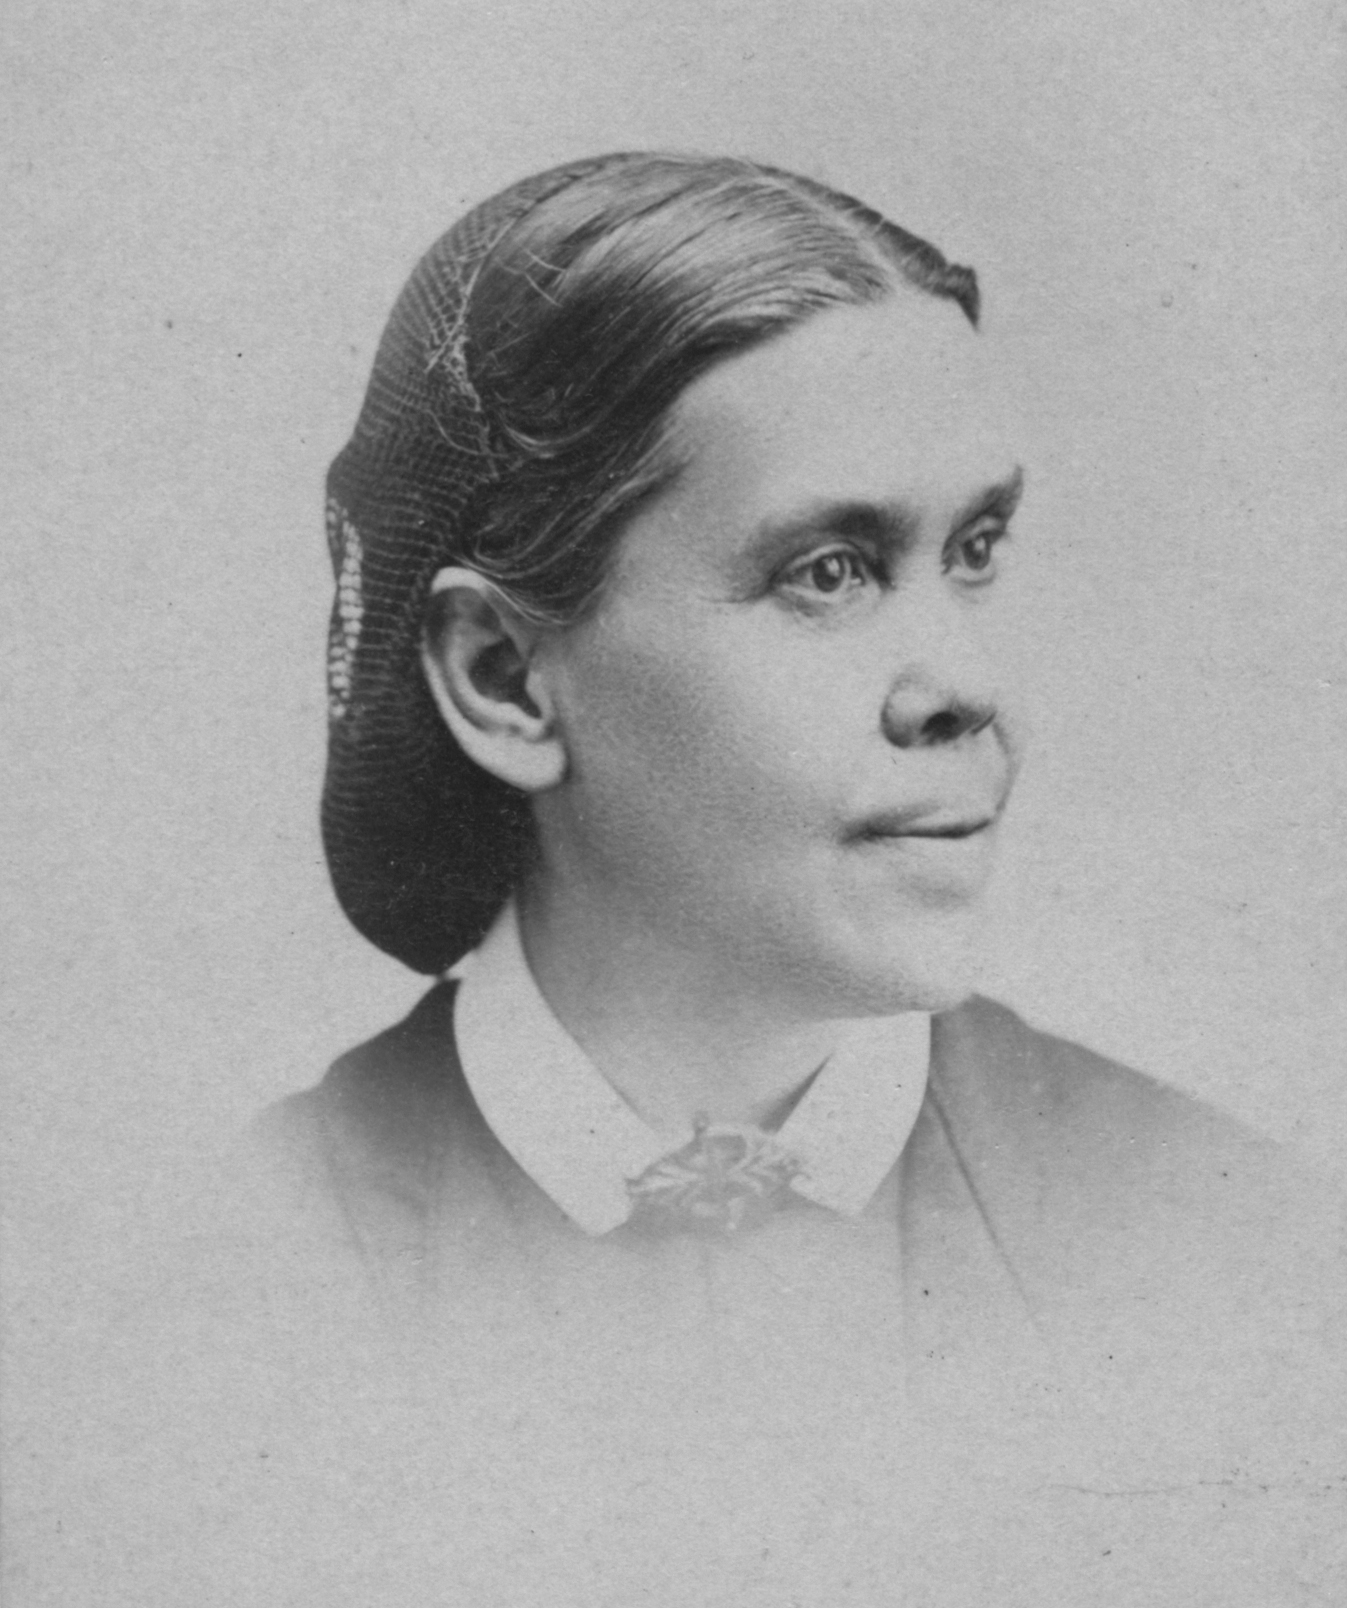
\includegraphics[width=0.65\linewidth]{images/ellen-white.jpg}
    \caption*{Ellen G. White}
    \label{fig:ellen-g-white}
\end{figure}


\begin{figure}[t]
    \centering
    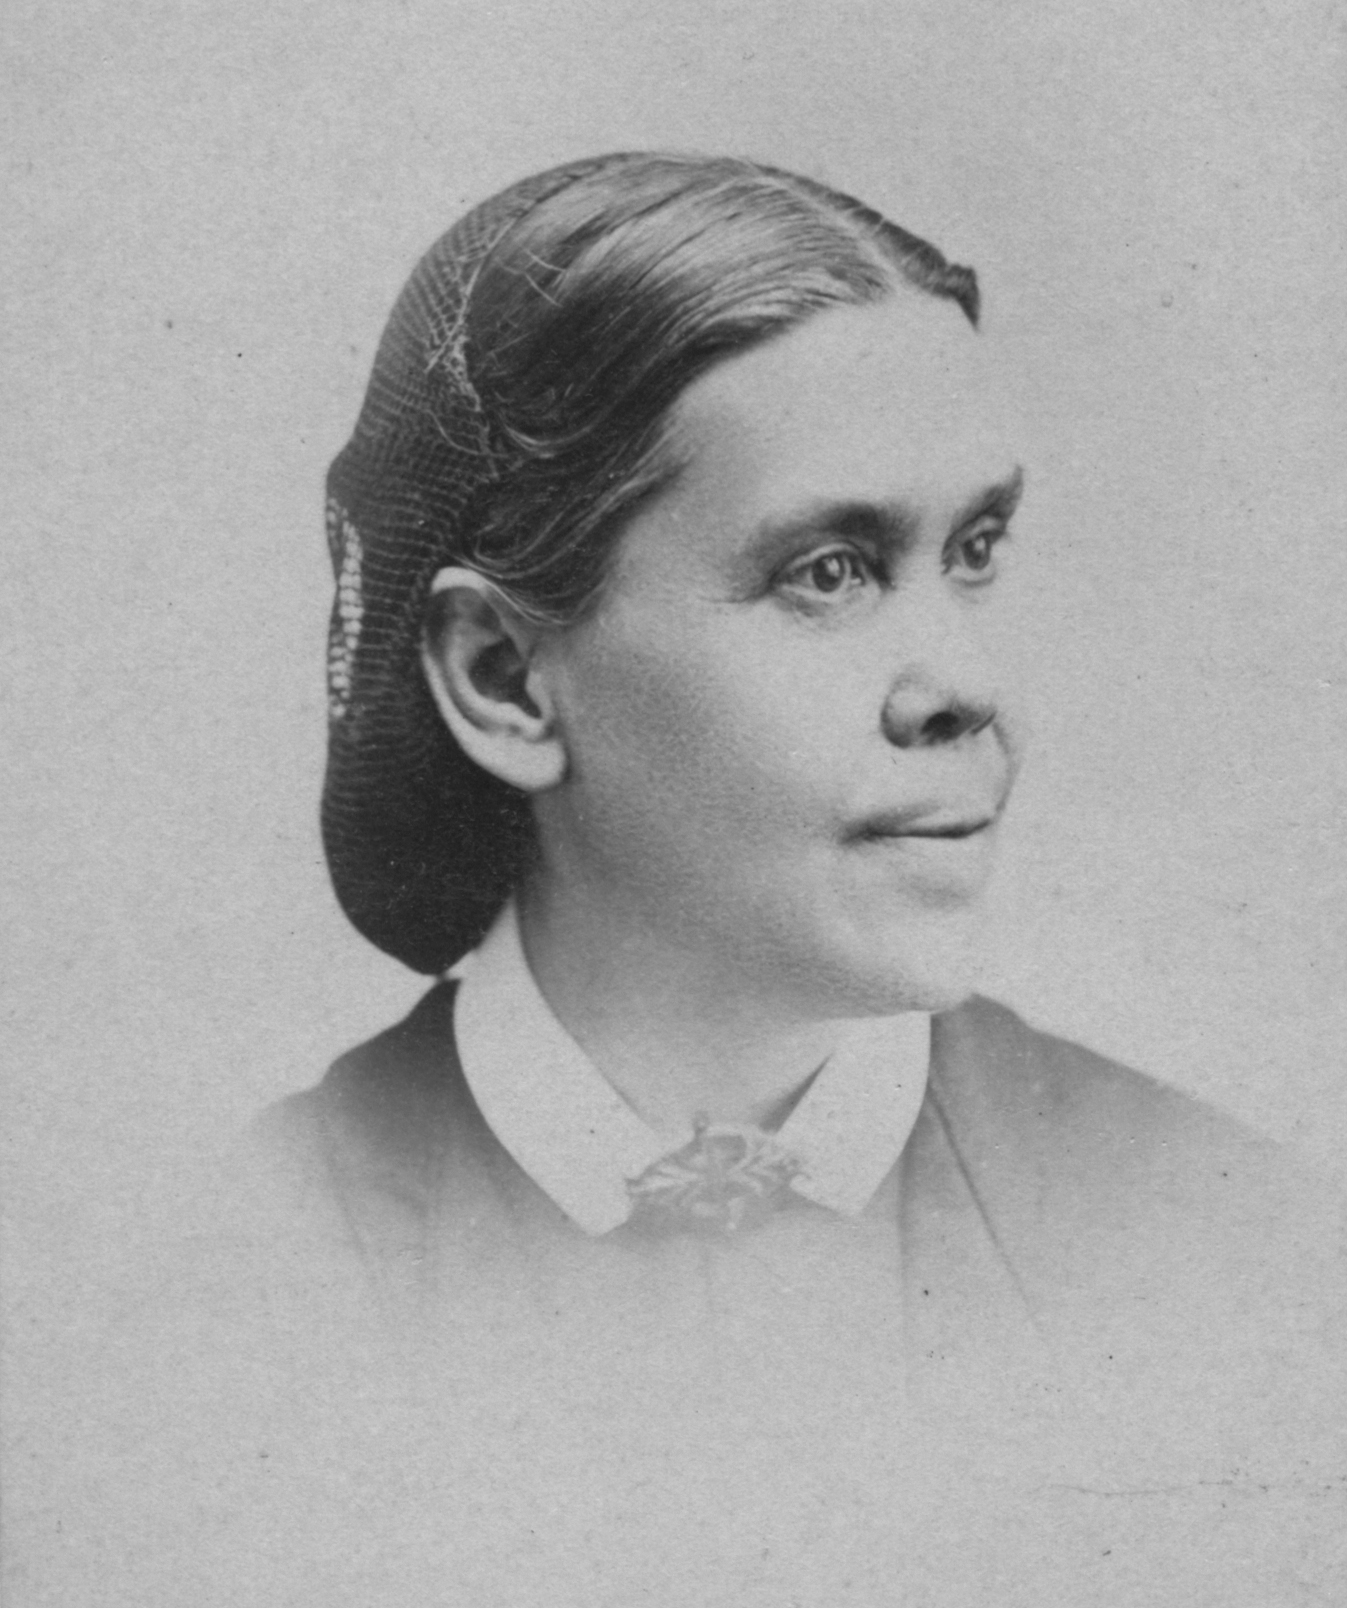
\includegraphics[width=0.65\linewidth]{images/ellen-white.jpg}
    \caption*{إلين ج. وايت}
    \label{fig:ellen-g-white}
\end{figure}


Consider the first point of the \emcap{Fundamental Principles}, which states that Seventh-day Adventists believe in \others{one God, \textbf{a personal, spiritual being}.}[First point of the Fundamental Principles][https://forgotten-pillar.s3.us-east-2.amazonaws.com/A+declaration+of+the+fundamental+principles+taught+and+practiced+by+the+Seventh-day+Adventists++.pdf] This makes it clear that the central issue in the doctrine of the \emcap{personality of God} concerns the outward, bodily form of the Father. But why was this such a vital and significant question? What were the implications of God having a bodily, personal form?


ضع في اعتبارك النقطة الأولى من \emcap{المبادئ الأساسية}، التي تنص على أن الأدفنتست السبتيين يؤمنون بـ \others{إله واحد، \textbf{كائن شخصي روحي}.}[النقطة الأولى من المبادئ الأساسية][https://forgotten-pillar.s3.us-east-2.amazonaws.com/A+declaration+of+the+fundamental+principles+taught+and+practiced+by+the+Seventh-day+Adventists++.pdf] هذا يوضح أن القضية المركزية في عقيدة \emcap{شخصانية الله} تتعلق بالشكل الخارجي، الجسدي للآب. ولكن لماذا كان هذا سؤالاً حيويًا ومهمًا؟ ما هي تداعيات امتلاك الله لشكل جسدي وشخصي؟


\othersQuote{But because the pioneers of the Seventh-day Adventist Church held that prophecy was fulfilled on October 22, 1844, and that an important work began in heaven in the Most Holy Place of the heavenly sanctuary at that time, and because the Adventists who had become \textbf{spiritualizers} took the position that Christ had come into their hearts on October 22, 1844, and that His kingdom was in their hearts, the founders of the church, and notably Ellen White, were classed by the world generally, and also by those that SDAs have termed first-day Adventists, as one and the same group. Here again the great enemy cast aspersion upon the true, paralleling it with a false, spurious experience.}[ALW, 1BIO 80.2; 1985][https://egwwritings.org/read?panels=p668.587]


\othersQuote{ولكن لأن رواد كنيسة الأدفنتست السبتيين اعتقدوا أن النبوة قد تحققت في 22 أكتوبر 1844، وأن عملاً مهماً بدأ في السماء في قدس الأقداس في المقدس السماوي في ذلك الوقت، ولأن الأدفنتست الذين أصبحوا \textbf{روحانيون} اتخذوا موقفاً بأن المسيح قد دخل قلوبهم في 22 أكتوبر 1844، وأن ملكوته في قلوبهم، فإن مؤسسي الكنيسة، وخاصة إلين وايت، تم تصنيفهم من قبل العالم بشكل عام، وأيضاً من قبل أولئك الذين أطلق عليهم الأدفنتست السبتيون أدفنتست اليوم الأول، كمجموعة واحدة. وهنا مرة أخرى ألقى العدو العظيم افتراءً على الحقيقي، موازياً إياه بتجربة زائفة ومزيفة.}[ALW, 1BIO 80.2; 1985][https://egwwritings.org/read?panels=p668.587]


\othersQuoteNoGap{Ellen White was to speak of this matter again, particularly in the closing paragraphs of her first little book, Experience and Views, published in 1851. As one reads this he will note the use of \textbf{the term spiritualism}, which must be taken in the light of the work of the spiritualizers and not in the light of what today is understood to be spiritualism or spiritism, although both emanate from the same source.}[ALW, 1BIO 80.3; 1985][https://egwwritings.org/read?panels=p668.588]


\othersQuoteNoGap{كان على إلين وايت أن تتحدث عن هذا الأمر مرة أخرى، خاصة في الفقرات الختامية من كتابها الصغير الأول، “الخبرة والرؤى”، الذي نُشر عام 1851. عندما يقرأ المرء هذا سيلاحظ استخدام \textbf{مصطلح الروحانية}، الذي يجب أن يُفهم في ضوء عمل الروحانيين وليس في ضوء ما يُفهم اليوم على أنه الروحانية أو استحضار الأرواح، على الرغم من أن كليهما ينبعان من نفس المصدر.}[ALW, 1BIO 80.3; 1985][https://egwwritings.org/read?panels=p668.588]


\othersQuoteNoGap{We turn now to the statement written and published in 1851 as found in Ibid., 77, 78:}[ALW, 1BIO 80.4; 1985][https://egwwritings.org/read?panels=p668.589]


\othersQuoteNoGap{نتجه الآن إلى البيان المكتوب والمنشور في عام 1851 كما ورد في المرجع نفسه، 77، 78:}[ALW, 1BIO 80.4; 1985][https://egwwritings.org/read?panels=p668.589]


\othersQuoteNoGap{\textbf{I have frequently been falsely charged with teaching views peculiar to Spiritualism}. But before the editor of The Day-Star ran into that delusion, \textbf{the Lord \underline{gave me a view} of the sad and desolating effects that would be produced upon the flock by him and others \underline{in teaching the spiritual views}}.}[ALW, 1BIO 80.5; 1985][https://egwwritings.org/read?panels=p668.590]


\othersQuoteNoGap{\textbf{لقد اتُهمت كثيراً زوراً بتعليم آراء خاصة بالروحانية}. ولكن قبل أن ينزلق محرر ذا داي-ستار في ذلك الضلال، \textbf{الرب \underline{أعطاني رؤية} عن الآثار المحزنة والمدمرة التي ستنتج على القطيع من خلاله ومن خلال آخرين \underline{في تعليم الآراء الروحانية}}.}[ALW, 1BIO 80.5; 1985][https://egwwritings.org/read?panels=p668.590]


\othersQuoteNoGap{I have often seen the lovely \textbf{Jesus, that He is a person}. I asked Him \textbf{\underline{if His Father was a person} and \underline{had a form} like Himself}. Said Jesus, ‘I am in \textbf{the express image of My Father’s person}.}[ALW, 1BIO 80.6; 1985][https://egwwritings.org/read?panels=p668.591]


\othersQuoteNoGap{لقد رأيت كثيراً يسوع الجميل، \textbf{أنه شخص}. سألته \textbf{\underline{إذا كان أبوه شخصاً} و\underline{له هيئة مثله}}. قال يسوع: ‘أنا \textbf{صورة جوهره}.}[ALW, 1BIO 80.6; 1985][https://egwwritings.org/read?panels=p668.591]


\othersQuoteNoGap{\textbf{I have often seen that \underline{the spiritual view} took away all the glory of heaven, and that in many minds the throne of David and the lovely person of Jesus have been burned up in the fire of Spiritualism.} I have seen that some who have been deceived and led into this error will be brought out into the light of truth, but it will be almost impossible for them to get entirely rid of \textbf{the deceptive power of Spiritualism}. Such should make thorough work in confessing their errors and leaving them forever.}[ALW, 1BIO 80.7; 1985][https://egwwritings.org/read?panels=p668.592]


\othersQuoteNoGap{\textbf{لقد رأيت كثيراً أن \underline{النظرة الروحانية} أزالت كل مجد السماء، وأنه في أذهان كثيرة تم حرق عرش داود وشخص يسوع الجميل في نار الروحانية.} لقد رأيت أن بعض الذين خُدعوا وقيدوا إلى هذا الخطأ سيُخرجون إلى نور الحق، ولكن سيكون من المستحيل تقريباً بالنسبة لهم التخلص تماماً من \textbf{القوة المخادعة للروحانية}. على هؤلاء أن يقوموا بعمل شامل في الاعتراف بأخطائهم وتركها إلى الأبد.}[ALW, 1BIO 80.7; 1985][https://egwwritings.org/read?panels=p668.592]


\othersQuoteNoGap{\textbf{The spiritualization of heaven, God, Christ, and the coming of Christ lay at the foundation of much of the fanatical teachings that 17-year-old Ellen Harmon was called upon by God to meet in those formative days. The visions firmly established \underline{the personality of God and Christ}, \underline{the reality of heaven} and the reward to the faithful, and the resurrection. This sound guidance saved the emerging church}.}[ALW, 1BIO 81.1; 1985][https://egwwritings.org/read?panels=p668.595]


\othersQuoteNoGap{\textbf{إن روحنة السماء والله والمسيح ومجيء المسيح كانت في أساس الكثير من التعاليم المتعصبة التي دُعيت إلين هارمون ذات السبعة عشر عاماً من قبل الله لمواجهتها في تلك الأيام التكوينية. أرست الرؤى بثبات \underline{شخصانية الله والمسيح}، \underline{وواقعية السماء} والمكافأة للأمناء، والقيامة. هذا التوجيه السليم أنقذ الكنيسة الناشئة}.}[ALW, 1BIO 81.1; 1985][https://egwwritings.org/read?panels=p668.595]


The mistake of the Millerite movement in 1844 lay in misunderstanding the nature of the event, not its timing. Daniel 7:13-14 describes Christ coming to the Ancient of Days in heaven to receive dominion, glory, and a kingdom—not His second coming to earth. This event, marking the beginning of Christ’s work in the Most Holy Place, occurred at the conclusion of the 2300-day prophecy in 1844. Unlike other Adventist groups, the emerging Seventh-day Adventist Church uniquely recognized this heavenly event.


إن خطأ حركة ميلر في عام 1844 كان في سوء فهم طبيعة الحدث، وليس توقيته. يصف دانيال 7:13-14 مجيء المسيح إلى القديم الأيام في السماء ليتسلم السلطان والمجد والملكوت - وليس مجيئه الثاني إلى الأرض. هذا الحدث، الذي يشير إلى بداية عمل المسيح في قدس الأقداس، حدث في نهاية نبوة الـ 2300 يوم في عام 1844. على عكس مجموعات الأدفنتست الأخرى، فإن كنيسة الأدفنتست السبتيين الناشئة تعرفت بشكل فريد على هذا الحدث السماوي.


This understanding is built on key premises:
\begin{itemize}
    \item Heaven is a real, literal place (John 14:1-3).
    \item There is a literal sanctuary in heaven where Christ ministers (Hebrews 8:2). 
    \item A real, physical throne exists in this sanctuary, occupied by God Himself (Daniel 7:9-10; Revelation 4:2-3; Ezekiel 1:26-28; Psalm 11:4).
\end{itemize}


يستند هذا الفهم على مقدمات رئيسية:
\begin{itemize}
    \item السماء هي مكان حقيقي وحرفي (يوحنا 14:1-3).
    \item هناك مقدس حرفي في السماء حيث يخدم المسيح (عبرانيين 8:2).
    \item يوجد عرش حقيقي ومادي في هذا المقدس، يشغله الله نفسه (دانيال 7:9-10؛ رؤيا 4:2-3؛ حزقيال 1:26-28؛ مزمور 11:4).
\end{itemize}


Why is the question of the Father’s bodily form so important? If God were not a physical being, there would be no need for a literal throne, sanctuary, or heavenly ministry. A spiritualized interpretation undermines the foundation of Seventh-day Adventist theology, leading to a domino effect that erodes the doctrine of Christ’s priestly work.


لماذا تعتبر مسألة هيئة الآب الجسدية مهمة جداً؟ إذا لم يكن الله كائناً مادياً، فلن تكون هناك حاجة لعرش حرفي أو مقدس أو خدمة سماوية. إن التفسير الروحاني يقوض أساس لاهوت الأدفنتست السبتيين، مما يؤدي إلى تأثير الدومينو الذي يآكل عقيدة عمل المسيح الكهنوتي.


The doctrine of the \emcap{personality of God} was a simple yet foundational teaching, affirmed in the first point of the \emcap{Fundamental Principles}: \textit{“One God, a personal, spiritual being.”} As such, He is not omnipresent by Himself but through His representative, the Holy Spirit.\footnote{The first point of the Fundamental Principles: \othersQuote{That there is \textbf{one God}, \textbf{a \underline{personal, spiritual being}}, the creator of all things, omnipotent, … and \textbf{everywhere present by \underline{his representative}, the Holy Spirit}. Ps. 139:7.}} When Ellen White asked Jesus \egwinline{if His Father \textbf{was a person} and \textbf{had a \underline{form}} like Himself,}[EW 77.1; 1882][https://egwwritings.org/read?panels=p28.490&index=0] we see clearly that the \textit{outward bodily \textbf{form}} is \textit{the quality or state} defining God as a person. This understanding was central in addressing the Kellogg crisis regarding \textit{The Living Temple}, which deviated from this core belief.


كانت عقيدة \emcap{شخصانية الله} تعليمًا بسيطًا لكنه أساسي، تم تأكيده في النقطة الأولى من \emcap{المبادئ الجوهرية}: \textit{“إله واحد، كائن شخصي روحي.”} وبهذه الصفة، فهو ليس حاضرًا في كل مكان بذاته ولكن من خلال ممثله، الروح القدس.\footnote{النقطة الأولى من المبادئ الجوهرية: \othersQuote{أن هناك \textbf{إله واحد}، \textbf{\underline{كائن شخصي روحي}}، خالق كل الأشياء، قدير، ... و\textbf{حاضر في كل مكان من خلال \underline{ممثله}، الروح القدس}. مز 139: 7.}} عندما سألت إلين وايت يسوع \egwinline{إذا كان أبوه \textbf{شخصًا} و\textbf{له \underline{هيئة}} مثله،}[EW 77.1; 1882][https://egwwritings.org/read?panels=p28.490&index=0] نرى بوضوح أن \textit{\textbf{الهيئة} الجسدية الخارجية} هي \textit{الصفة أو الحالة} التي تعرّف الله كشخص. كان هذا الفهم محوريًا في معالجة أزمة كيلوغ بخصوص \textit{ذا ليفينغ تمبل}، الذي انحرف عن هذا المعتقد الأساسي.


But do our current \textit{Fundamental Beliefs} still affirm this doctrine? Do they explicitly teach that God is a real person with a bodily form, whose literal presence is in heaven, while He is omnipresent through His Spirit? The doctrine of God’s presence and personality is absent from today’s official beliefs. While individually, we may still believe in it, why was such a vital teaching omitted? What were the reasons behind this shift? These are the questions we must explore further in the context of \textit{The Foundation of Our Faith}.


لكن هل لا تزال \textit{المعتقدات الأساسية} الحالية تؤكد هذه العقيدة؟ هل تعلّم صراحةً أن الله شخص حقيقي له هيئة جسدية، وأن حضوره الحرفي في السماء، بينما هو حاضر في كل مكان من خلال روحه؟ إن عقيدة حضور الله وشخصانيته غائبة عن المعتقدات الرسمية اليوم. بينما قد نؤمن بها فرديًا، لماذا تم حذف مثل هذا التعليم الحيوي؟ ما هي الأسباب وراء هذا التحول؟ هذه هي الأسئلة التي يجب أن نستكشفها بشكل أعمق في سياق \textit{أساس إيماننا}.


% The Historical Context

\begin{titledpoem}
    
    \stanza{
        By visions Ellen White stood firm, \\
        Against false views; she did affirm. \\
        The Father’s form, a truth profound, \\
        In this essential faith was found.
    }

    \stanza{
        "Spiritualizers" sought to claim \\
        That heaven’s realm was but a name. \\
        Yet God has form, like Christ His Son, \\
        This truth our founders built upon.
    }

    \stanza{
        A Spirit Person God does reign \\
        The universe is His domain \\
        This doctrine once our cornerstone, \\
        Has somehow from our statements flown.
    }
    
\end{titledpoem}